% !TeX root = ../libro.tex
% !TeX encoding = utf8

\chapter{Implementación}\label{Implementacion}
El código se ha desarrollado usando el software \textit{Jupyter Notebook} en el lenguaje \textit{Python}, concretamente en su versión 3 \cite{10.5555/1593511}. La ventaja de \textit{Jupyter Notebook} para este trabajo es su estructura visual con céldas y texto, la fácil implementación y ejecución del código en \textit{Python} y que el resultado de las ejecuciones se queda grabado justo debajo de la celda ejecutada. Esto último es útil para la entrega del software, pues el conjunto de datos es privado y no puede entregarse y por tanto, hay que solicitar permiso para obtener los datos y ejecutar el código. Sin embargo, con Jupyter pueden verse los resultados de cada celda sin la necesidad de ejecutarlo.\\
El código se estructura en seis partes:
\begin{itemize}
  \item Exploración con datos de tríos: En esta primera exploración se han utilizado sólo los datos de la familia (sin los datos de control) para la experimentación.
  \item Primeros datos de control: Se han utilizado los padres del conjunto de tríos y se han juntado con los primeros datos de control para repetir la experimentación.
  \item Segundos datos de control: Padres y segundos datos de control para verificar los resultados obtenidos con los primeros controles.
  \item Diferencias entre ambos controles: Ambos conjuntos de datos de control para detectar sus diferencias.
  \item Selección de variables: Apartado con selección de variables, reducción de dimensionalidad y reentrenamiento de modelos.
  \item Diferencias de sesgo: Apartado con dos tests para comprobar las diferencias entre los conjuntos de datos debidas al sesgo del laboratorio.
\end{itemize}
El objetivo del programa es la detección de sesgo de laboratorio en datos genéticos, concretamente en datos genéticos de intensidades de SNPs con una estructura de carpetas y columnas definida en la \autoref{st:Materiales}. Este sesgo puede deberse a diferencias en la cantidad de reactivo usado en cada experimento o en los tiempos de reacción ya que el genotipado se basa en la PCR que genera una replicación exponencial de la información genética de cada individuo que va a ser extraída. Además el programa calcula tests para medir la significación de ese sesgo, es decir, si las diferencias detectadas son aleatorias o es sesgo real, es decir, existe un patrón común a los SNPs que puede estar indicando un sesgo de laboratorio o del experimento.\\
El programa detecta el sesgo entre tres conjuntos de datos (tríos y los dos de control) mediante modelos de aprendizaje automático que clasifican los datos.

\section{Paquetes utilizados}
En esta sección se repasarán los paquetes que han sido necesarios incluir para la realización del código en \textit{Python}.\\
Los paquetes que se han utilizado en el trabajo son los siguientes:
\begin{itemize}
\itemsep 0em 
  \item \textit{scikit-learn} \cite{scikit-learn}: Es un paquete desarrollado específicamente para el aprendizaje automático en \textit{Python} y es más utilizado en el código desarrollado. Se han usado distintos clasificadores, métricas y preprocesado de \textit{datasets}.
  \item \textit{pandas} \cite{mckinney-proc-scipy-2010}: Librería utilizada para la representación de datos. Es un paquete desarrollado para tratar, manipular y analizar datos con facilidad.
  \item \textit{matplotlib} \cite{Hunter:2007}: Paquete para la creación de diversos tipos de gráficas, animaciones y visualizaciones interactivas en \textit{Python}. En este trabajo se ha utilizado para la creación de diferentes gráficos.
  \item \textit{scipy} \cite{scipy}: Es un paquete de código abierto desarrollado para ingeniería, matemáticas y ciencia. En este trabajo lo usamos para los tests de Wilcoxon y el T-Test.
\end{itemize}

\section{Exploración de los datos}
En las cuatro primeras secciones del código, se ha realizado una exploración de los datos sin ningún tipo de selección de variables o reducción de dimensionalidad.
En la representación de los datos se ha usado un \textit{dataframe} del paquete \textit{pandas} \cite{mckinney-proc-scipy-2010}, dejando como nombre de las filas el ID del individuo correspondiente y como nombre de las columnas o variables, se ha establecido el nombre del SNP, tanto para el alelo A como para el B.
\subsection{Conjunto de datos de tríos y primer control}
Antes que nada se ha realizado un estudio de la base de datos de tríos en el que no esperamos encontrar diferencias significativas, dado que los estudios del GWAS realizados con estos datos no obtuvieron buenos resultados \cite{szatmari2007mapping}, pero era necesario intentar diferenciar padres de hijos afectados y nos dará una idea de cómo son los datos y cómo llegan a comportase los modelos.
Para empezar, se han leído sólo los datos de tríos mediante el paquete \textit{pandas} \cite{mckinney-proc-scipy-2010} para leer tanto los datos como los nombres de las columnas. Los nombres de las columnas (nombres de las variables) se han repetido para que las parejas de columnas de valores de SNPs tengan el mismo nombre y se ha añadido tanto el Género como el ID familiar para seguir el formato de los datos explicado en el \autoref{Conjunto}. Para los datos, se han eliminado todas las columnas de IDs excepto el familiar debido a que si no se eliminaran, los modelos harían una predicción perfecta sólo basándose en si el sujeto tiene ID de padre y madre (es decir, es un hijo y es afectado) o no (es padre y es sano). Se ha dejado el género para que el modelo lo tenga en cuenta pues en la herencia genética el género es influyente, así como el ID familiar para que se relacionen los tres individuos de una familia.\\
Después se ha separado en conjuntos train (entrenamiento) y test usando un 25\% de los individuos para el test y un 75\% para el train manteniendo la proporción entre sanos y enfermos y se han contabilizado cuántos individuos hay en cada conjunto quedando 438 sanos y 210 afectados en el test y 1290 sanos y 654 afectados en el conjunto de entrenamiento, con un total de 1944 instancias en train y 648 en test.\\
También para realizar un acercamiento más visual a los datos se han representado las intensidades de dos SNPs. En el eje de abscisas está el valor de la primera columna A para el SNP y en el de ordenadas el valor de la segunda columna B. No se ha modificado el valor de las intensidades de ninguna forma, están directamente representadas en la gráfica. Podemos ver dos colas, dos líneas en la gráfica que representan los individuos homocigóticos y heterocigóticos. También podemos apreciar que las intensidades no están en forma de punto sino de línea reflejando la naturaleza exponencial de la \textit{Polymerase Chain Reaction} (PCR), mostrando inviduos con intensidad total ($intensidad_{AB}=intensidad_{A}+intensidad_{B}$) muy baja y otros mucho más alta. La gráfica se ha dibujado mediante la librería \textit{matplotlib} \cite{Hunter:2007}.

\begin{figure}[H]
\centering
\begin{minipage}{.5\textwidth}
  \centering
  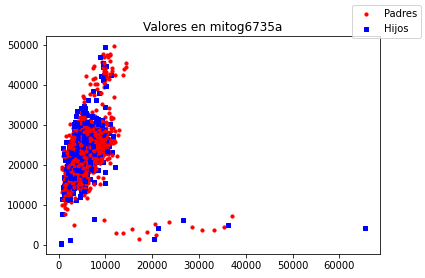
\includegraphics[width=.8\linewidth]{trios_snp1}
  \captionof{figure}{SNP mitog6735a en tríos.}
  \label{fig:snp1-trios}
\end{minipage}%
\begin{minipage}{.5\textwidth}
  \centering
  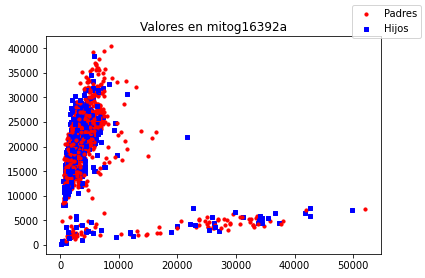
\includegraphics[width=.8\linewidth]{trios_snp2}
  \captionof{figure}{SNP mitog16392a en tríos.}
  \label{fig:snp2-trios}
\end{minipage}
\end{figure}

Visualmente se podría decir que es difícil ver diferencias entre padres e hijos.\\\\

El siguiente paso fue intentar predecir si los padres iban a tener un hijo afectado quitando los individuos hijos de la base de datos de tríos, marcando los padres como afectados y añadiendo los individuos de control al conjunto marcados como sanos. También es necesario borrar dos SNPs, cuatro variables en el conjunto, que hay de más en los datos de tríos. En concreto son los SNPs mitoc10874t y mitog10590a.\\
El número de instancias total que queda en el conjunto es de 4427 y 273 variables. Se ha partido en conjuntos de entrenamiento (75\%) y test (25\%) quedando 3320 instancias en el entrenamiento con 2040 individuos sanos y 1280 padres de individuos afectados y en el test 1107 con 659 individuos sanos y 448 padres de afectados.\\
Visualmente se han representado dos SNPs con los valores del alelo A en el eje x y los del alelo B en el y para cada individuo.

\begin{figure}[H]
\centering
\begin{minipage}{.5\textwidth}
  \centering
  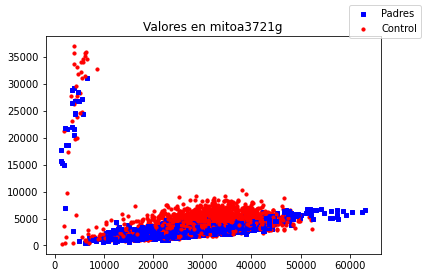
\includegraphics[width=.8\linewidth]{control1_snp1}
  \captionof{figure}{SNP mitoa3721g primer control.}
  \label{fig:snp1-control1}
\end{minipage}%
\begin{minipage}{.5\textwidth}
  \centering
  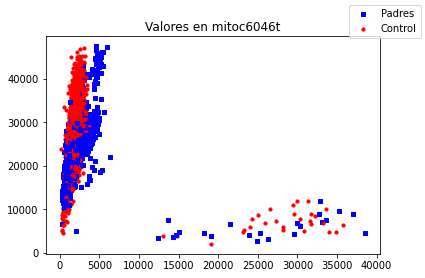
\includegraphics[width=.8\linewidth]{control1_snp2}
  \captionof{figure}{SNP mitoc6046t primer control.}
  \label{fig:snp2-control1}
\end{minipage}
\end{figure}

Se puede ver a simple vista que las diferencias van a ser mucho más fáciles de encontrar que en la base de datos de tríos. Diferencias que van a darse por el genotipado (en los arrays usados) que hacen que no puedan compararse directamente.

\subsection{Segundo conjunto de control}
En el caso de los segundos datos de control se ha juntado con los datos de los tríos de la misma forma que con el primer control: se han eliminado los individuos afectados (hijos) de los datos de familias y se han marcado a los padres como afectados. Después se han eliminado los SNPs redundantes de los padres y se han juntado con estos segundos datos de control. Por último, se ha separado en conjuntos de entrenamiento y test en un 75\% y 25\% respectivamente quedando de las 4648 instancias totales, 3486 para el conjunto \textit{train} (2211 sanos y 1275 padres de afectados) y 1162 para el test (con 709 sanos y 453 padres de afectados). Hay un desbalanceo de datos con 2920 individuos sanos y 1728 padres de afectados.\\
Se han representado dos SNPs con sus dos alelos A y B en el eje de abscisas y ordenadas respectivamente:

\begin{figure}[H]
\centering
\begin{minipage}{.5\textwidth}
  \centering
  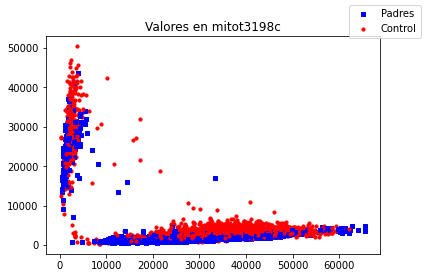
\includegraphics[width=.8\linewidth]{control2_snp1}
  \captionof{figure}{SNP mitot3198c segundo control.}
  \label{fig:snp1-control1}
\end{minipage}%
\begin{minipage}{.5\textwidth}
  \centering
  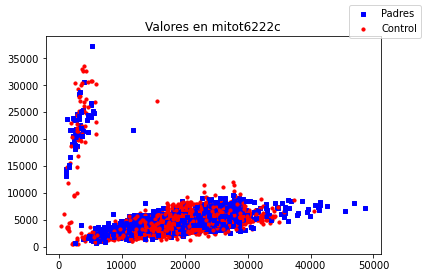
\includegraphics[width=.8\linewidth]{control2_snp2}
  \captionof{figure}{SNP mitot6222c segundo control.}
  \label{fig:snp2-control1}
\end{minipage}
\end{figure}

Los datos visualmente presentan cierta separación.

\subsection{Ambos datos de controles}
Para comprobar las diferencias de sesgo que haya podido haber por la extracción de los datos en laboratorio, se ha hecho también un estudio sobre ambos datos de control. Se ha leído de la misma forma que los anteriores apartados pero esta vez no hay SNPs redundantes y se han separado en conjuntos de entrenamiento y test en un 75\% y 25\%. También se ha marcado con la etiqueta 0 los datos del primer control y con 1 los del segundo.\\
Esta vez los datos están más balanceados quedando de los 5619 individuos totales, 2920 son del segundo control y 2699 del primero. Para el test quedan 714 del primer control y 691 del segundo y para el entrenamiento, 1985 del primer control y 2229 del segundo control. Se han representado de nuevo dos de los SNPs:

\begin{figure}[H]
\centering
\begin{minipage}{.5\textwidth}
  \centering
  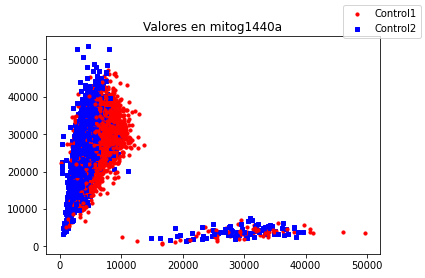
\includegraphics[width=.8\linewidth]{controles_snp1}
  \captionof{figure}{SNP mitog1440a dos controles.}
  \label{fig:snp1-control1}
\end{minipage}%
\begin{minipage}{.5\textwidth}
  \centering
  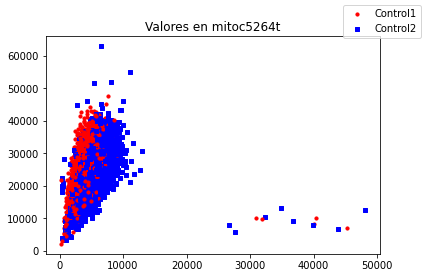
\includegraphics[width=.8\linewidth]{controles_snp2}
  \captionof{figure}{SNP mitoc5264t dos controles.}
  \label{fig:snp2-control1}
\end{minipage}
\end{figure}

Los controles, como se puede comprobar en un primer vistazo, están bien diferenciados, lo que apunta a diferencias de sesgo debidas a la extracción de los datos en laboratorio.

\section{Preprocesado de datos y selección de variables}\label{preprocesado}
En general, en los modelos se ha trabajado con los datos \textit{en crudo} (esto es, sin transformar ni seleccionar variables) excepto para el \textit{GridSearch CV} que explicaremos más adelante y para la parte de selección de variables.\\
Las transformaciones de los datos que se han realizado para ejecutar el mencionado \textit{GridSearch CV} han sido tres:
\begin{itemize}
  \item \textbf{Variance Threshold}: De la librería \textit{sklearn} \cite{scikit-learn}, elimina todos las características que no superan cierto umbral (\textit{threshold} en inglés). Esto se hace para eliminar características muy parecidas y aporten más complejidad que información a los datos. Se ha usado el valor $0.01$.
  \item \textbf{StandardScaler}: Estandariza los datos eliminando la media y escalando a varianza unidad. El valor del estandarizado en una observación $x$ se calcula como $z=\frac{x-u}{s}$, donde $u$ es la media de la muestra de entrenamiento y $s$ es la desviación estándar de la muestra de entrenamiento. También usado de la librería \textit{sklearn}.
  \item \textbf{PolynomialFeatures}: Añade una nuema matriz de calacterísticas de combinaciones de las características existentes con grado menor o igual que el indicado por parámetro, en este caso $2$. Se usa para cambiar la distribución de probabilidad separando más valores pequeños y grandes. De nuevo, usando el implementado por \textit{sklearn}.
\end{itemize}
También en el apartado de selección de variables para una reducción de dimensionalidad. Se empieza por una matriz de correlación para ver visualmente las posibles correlaciones entre variables mediante el método \texttt{corr} de \texttt{LabelEncoder} de la librería \textit{sklearn} y tras ello, lanzamos dos tests para la selección y ajustamos dos modelos para seleccionar las variables que nos indiquen.\\
Los dos test son el test $\chi^2$ de independencia y el de \textit{VarianceThreshold} explicado anteriormente. La hipótesis nula del test $\chi^2$ es que las variables son idependientes de sus etiquetas, con lo que si nos devuelve un p-valor mayor que $0.05$ aceptamos esta hipótesis y eliminamos esta variable del conjunto ya que no nos aporta al entrenamiento por ser idependiente del etiquetado que deseamos.\\
Los dos modelos entrenados para realizar la selección son \textit{LinearSVC} y \textit{ExtraTreesClassifier}, estos modelos se entrenan con el conjunto de entrenamiento y se seleccionan las variables que más hayan aportando al entrenamiento. En el primer modelo, se seleccionan las variables que tengan un aporte mayor a $10^{-5}$ por haber usado regularización L1 (especificado por parámetro al modelo) y en el segundo, los que estén por encima de la media (por defecto). Esta selección se lleva acabo con \texttt{SelectFromModel} de \textit{sklearn}.\\
El modelo \textit{LinearSVC} es un modelo de soporte vectorial como el que ya se ha explicado pero en su versión lineal, que permite la selección de variables. Se usan los parámetros $C=0.01$, regresión L1 y $dual=False$ que es preferible cuando hay más muestras que variables como en este caso \cite{scikit-learn}. Por otra parte el \textit{ExtraTreesClassifier} es un meta-modelo que lo que hace es entrenar cierto número de árboles de decisión aleatorios en varios subconjuntos de datos usando la media para mejorar el \textit{accuracy} y controlar el sobreajuste \cite{scikit-learn}. De parámetros se han escogido $50$ árboles.

\section{Modelos empleados y sus parámetros}
Describimos en esta sección la implementación de los modelos utilizados y los parámetros de los mismos para la clasificación.\\
Para evaluar cada modelo se ha dibujado \cite{Hunter:2007} la matriz de confusión para cada clasificador. La matriz representa el número de falsos y verdaderos positivos así como el de falsos y verdaderos negativos, se ha realizado con la librería \texttt{metrics} de \textit{scikit-learn} \cite{scikit2021metrics}, contando en forma de matriz $2x2$ las etiquetas que el modelo ha predicho y su verdadera etiqueta, como se explicó en la \autoref{Confusion}. Además, mediante el método \texttt{classification$\_$report} de \texttt{metrics} se han mostrado todas las métricas explicadas en la \autoref{Metricas} pasando por parámetro las etiquetas predichas por el modelo y las reales.
\subsection{Modelo K-NN}
Se ha utilizado la implementación del paquete \textit{scikit-learn} \cite{scikit2021knn}. En concreto, dentro del subpaquete \texttt{neighbours} el método \texttt{KNeighboursClassifier}. Se ha usado con los parámetros por defecto:
\begin{itemize}
\itemsep 0em 
  \item Número de vecinos: 5, es un modelo 5-NN.
  \item Pesos: Uniforme, todos los vecinos tienen la misma importancia.
  \item Métrica: Se usa la de Minkowski.
  \item p: 2, se usa la distancia euclídea.
\end{itemize}
Este modelo se ha entrenado para las partes de tríos y del primer control, dando una primera idea del rendimiento del resto de modelos sobre estos conjuntos. Normalmente su rendimiento es relativamente pobre pero como comentábamos en secciones anteriores, lo compensa con su baja complejidad y su alta entendibilidad.

\subsection{Regresión Logística}
Para la regresión logística (RL) he establecido que los pesos estén balanceados para contrarrestar el gran desbalanceo de los datos (hay el doble de padres, no afectados, que de hijos, afectados y muchos más de controles que de padres de afectados). Los parámetros utilizados han sido los siguientes \cite{scikit2021lr}:
\begin{itemize}
\itemsep 0em 
  \item \textit{Loss}: La función de pérdida, establecida a $log$ (función logística) para que el modelo sea aplique una regresión logística como la explicada en el \autoref{Aprendizaje}.
  \item \textit{penalty}: La regularización empleada. En este caso la L2 o de Ridge.
  \item \textit{alpha}: Parámetro que multiplica a la regularización, cuanto más alto, mayor será la regularización aplicada al modelo y menor el sobreajuste. Establecida por defecto a $0.0001$.
  \item \textit{class$\_$weight}: Pesos asociados con las variables. Se establecen como \textit{balanced}.
\end{itemize}
Se ha usado en su versión estocástica del subpaquete \texttt{linear$\_$model}, el método \texttt{SGDClassifier}. También se muestran los ceficientes resultantes del entrenamiento para cada variable mediante el método \texttt{coef$\_$} y se han mostrado las más influyentes, es decir, las que tienen mayor coeficiente, para la predicción.
\subsection{Árboles de decisión}
Estableciendo de nuevo los datos balanceados para reducir el desbalanceo que presentan estos conjuntos de datos, los parámetros establecidos para el modelo han sido los siguientes \cite{scikit2021dt}:
\begin{itemize}
\itemsep 0em 
  \item Criterio para medir la calidad de una división: Gini.
  \item Elegir la mejor división (parámetro \textit{splitter}=\textit{best})
  \item Mínimo 2 muestras para dividir un nodo
  \item Mínimo una muestra para ser un nodo hoja
\end{itemize}
Se muestran también como en regresión logística las variables más importantes a la hora de predecir. esto se hace mediante el método \texttt{feature$\_$importances$\_$} del modelo de \textit{DecisionTreeClassifier} de \textit{sklearn}.
\subsection{Máquinas de soporte vectorial}
Se han entrenado dos versiones de este modelo, para el conjunto de datos de tríos se han establecido los pesos balanceados y se han usado los valores por defecto y para los primeros datos de control se han cambiado varios parámetros para mejorar los resultados. La implementación usada es la de la librería de \textit{sklearn} \cite{scikit2021svm}. Los parámetros modificados son:
\begin{itemize}
\itemsep 0em 
  \item Parámetro C: Es el parámetro de regularización, cuanto mayor sea, menor es la regularización aplicada, es decir, son inversamente proporcionales. Por defecto es $1$ y se ha establecido a $100$.

\end{itemize}


\endinput
%------------------------------------------------------------------------------------
% FIN DEL CAPÍTULO. 
%------------------------------------------------------------------------------------









